\documentclass[russian,utf8,emptystyle]{eskdtext}

\newcommand{\No}{\textnumero} % костыль для фикса ошибки

\ESKDdepartment{Федеральное государственное бюджетное образовательное учреждение высшего профессионального образования}
\ESKDcompany{Московский государственный технический университет им. Н. Э. Баумана}
\ESKDclassCode{23 0102}
\ESKDtitle{АИС поиска алгоритмов распознавания изоморфизма графов с помощью генетического программирования}
\ESKDdocName{Руководство пользователя}
\ESKDauthor{Гуща~А.~В.}
%\ESKDtitleApprovedBy{~}{~\underline{\hspace{2.5cm}}}
%\ESKDtitleAgreedBy{~}{~\underline{\hspace{2.5cm}}}
\ESKDtitleDesignedBy{Студент группы ИУ5-82}{Гуща~А.~В}
 
\usepackage{multirow}
\usepackage{tabularx}
\usepackage{tabularx,ragged2e}
\renewcommand\tabularxcolumn[1]{>{\Centering}p{#1}}
\newcommand\abs[1]{\left|#1\right|}

\begin{document}
\maketitle
\tableofcontents
\newpage

\section{Назначение программы}
Назначением разработки является предоставлению пользователю инструментов по автоматическому поиску алгоритмов проверки изоморфизма ориентированных графов и выдача графической информации для осуществления ручного анализа.

\section{Условия выполнения программы}
\subsection{Требования к программным средствам}
Для работы данного приложения необходимо, чтобы на компьютере были установлены следующие программные продукты:
\begin{itemize}
\item Операционная система семейства GNU/Linux с версией ядра не ниже 3.0
\item Оконная система X Window System не ниже версии X11R7.3
\item Библиотеа элементов интерфейса GTK+ не ниже версии 3.10
\end{itemize}

\subsection{Требования к составу технических средств}
Данная программа должна работать на компьютере следующей конфигурации:
\begin{itemize}
\item Процессор, поддерживающий архитектуру x86\underline{~}64 с тактовой частотой не менее 1.5 ГГц
\item Оперативная память объемом не менее 1 Гб
\item Графический ускоритель и монитор, способные отображать графический интерфейс операционной системы
\item Устройства ввода: мышь и клавиатура
\end{itemize}

\subsection{Требования к подготовке оператора}
Для продуктивного использования данного программного продукта пользователь должен обладать следующими навыками и иметь компетенции:
\begin{itemize}
\item Базовые знания английского языка, если операционная система имеет английский язык как основной
\item Знания из теории графов: понятия графа, изоморфизма графов, деревья и др.
\item Базовые знания информатики: алгоритм, программа, процесс интерпретации, проблемно-ориентированный язык программирования и др.
\item Базовые знания эволюционных методов: функция приспособленности, популяция, индивиды, геном и др.
\end{itemize}

\section{Выполнение программы}
\subsection{Инсталляция программного продукта}
Для инсталляции программного продукта необходимо скопировать следующие файлы в инсталляционную папку:
\begin{itemize}
\item graph-isomorph
\item gui.glade
\item icon.png
\item icon-small.png
\end{itemize}

\subsection{Запуск программного продукат}
Для запуска программы необходимо произвести двойное нажатие левой клавиши мышки на иконке файла <<graph-isomorph>> в графическом режиме или через терминал: перейти в инсталляционную папку и ввести:
\begin{verbatim}
./graph-isomorph
\end{verbatim} 

Возможен запуск с заранее определенным файлом проекта: 
\begin{verbatim}
./graph-isomorph --proj=имя_файла_проекта
\end{verbatim}

Для получения справки о входных параметрах приложения:
\begin{verbatim}
./graph-isomorph --help
\end{verbatim}

Что отобразит в терминале следующее сообщение:
\begin{verbatim}
$ ./graph-isomorph --help
graph-isomorph [options]

options:  --gui=<path>  - path to glade file. Optional, default 
                          is 'gui.glade'.
          --log=<path>  - path to log file. Optional, default 
                          is 'graph-isomorph.log'.
          --proj=<path> - path to project file. Optional, default 
                          is './project.yaml'. 
          --help        - display the message.
\end{verbatim}

\newpage
\section{Сообщения оператору}
\subsection{Выход из приложения}
Чтобы осуществить выход из приложения, необходимо:
\begin{itemize}
\item Вызвать контекстное меню <<Файл>> нажатием левой клавиши мыши
\item Нажать на пункт <<Выход>> левой клавишей мыши
\end{itemize}

\begin{figure}[h!]
\centering
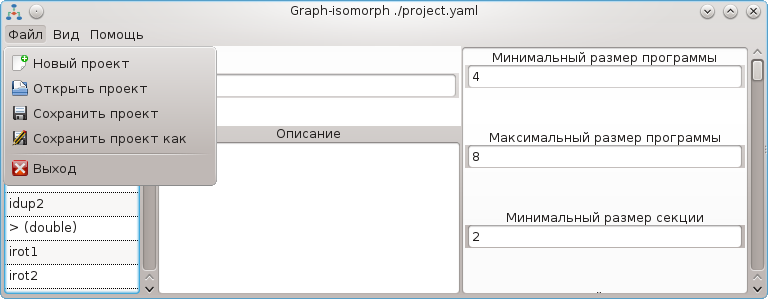
\includegraphics[width=0.8\textwidth]{screen01}
\caption{Выход из приложения}
\end{figure}

\subsection{Вызов справочной информации}
Чтобы просмотреть справочную ифнормацию, необходимо:
\begin{itemize}
\item Вызвать контекстное меню <<Помощь>> нажатием левой клавиши мыши
\item Нажать на пункт <<О программе>> левой клавишей мыши
\end{itemize}

\begin{figure}[h!]
\centering
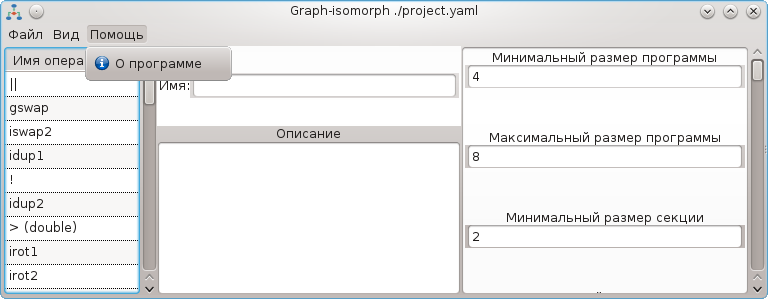
\includegraphics[width=0.8\textwidth]{screen02}
\caption{Вызов справочной информации}
\end{figure}

\begin{figure}[h!]
\centering
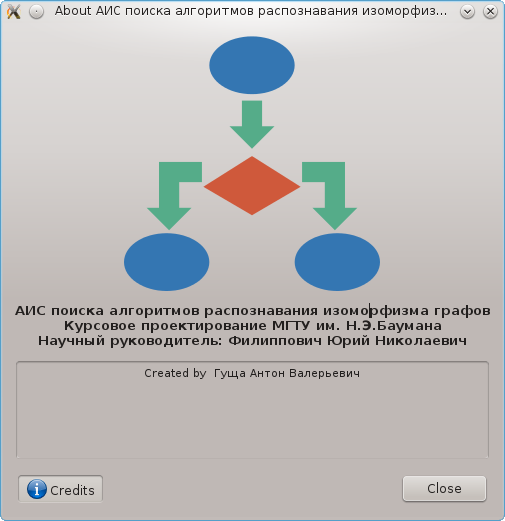
\includegraphics[width=0.5\textwidth]{screen03}
\caption{Просмотр справочной информации}
\end{figure}

\subsection{Операции с проектом}
Вся информация, которая должна передаваться между запусками приложения, хранится в \textbf{проекте}, который сохраняется на жесткий диск в формате YAML. По умолчанию открывается проект с именем <<project.yml>>.

\subsubsection{Создание нового проекта}
Для создания нового проекта необходимо:
\begin{itemize}
\item Вызвать контекстное меню <<Файл>> нажатием левой клавиши мыши
\item Нажать на пункт <<Новый проект>>
\item В появившемся диалоге <<Выберите файл нового проекта>> осуществить выбор файла
\item Нажать на кнопку <<OK>> диалога
\end{itemize}

\begin{figure}[h!]
\centering
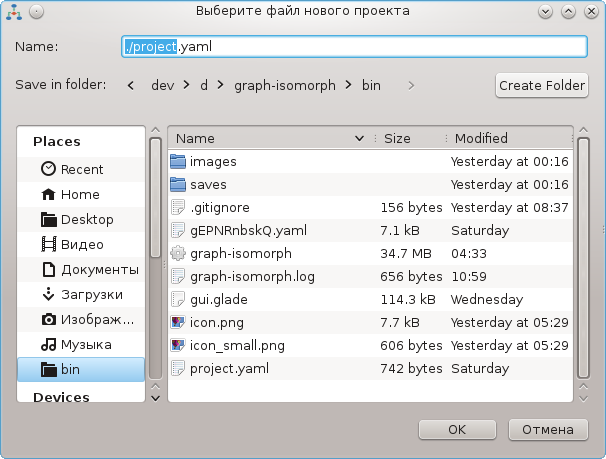
\includegraphics[width=0.5\textwidth]{screen04}
\caption{Диалог создания нового проекта}
\end{figure}

\subsubsection{Открытие проекта}
Для открытия проекта необходимо:
\begin{itemize}
\item Вызвать контекстное меню <<Файл>> нажатием левой клавиши мыши
\item Нажать на пункт <<Открыть проект>>
\item В появившемся диалоге <<Выберите файл проекта>> осуществить выбор файла
\item Нажать на кнопку <<OK>> диалога
\end{itemize}

\begin{figure}[h!]
\centering
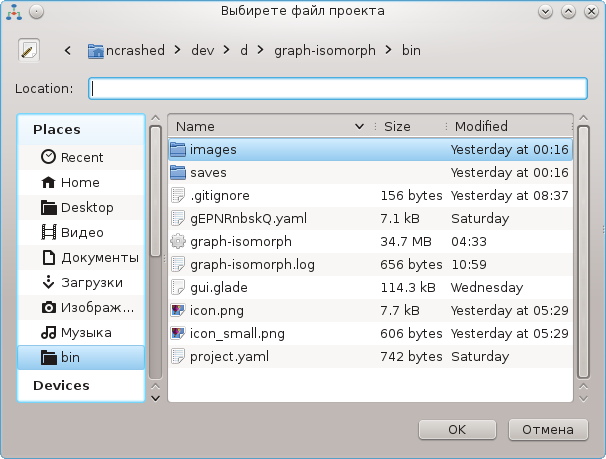
\includegraphics[width=0.5\textwidth]{screen05}
\caption{Диалог открытия проекта}
\end{figure}

\subsubsection{Сохранение проекта}
Есть два способа сохранения проекта:
\begin{itemize}
\item Сохранение по текущему названию проекта:
\begin{itemize}
\item Вызвать контекстное меню <<Файл>> нажатием левой клавиши мыши
\item Нажать на пункт <<Сохранить проект>>
\end{itemize}
\item Сохранение с уточнением названия проекта:
\begin{itemize}
\item Вызвать контекстное меню <<Файл>> нажатием левой клавиши мыши
\item Нажать на пункт <<Сохранить проект как>>
\item В появившемся диалоге <<Выберите файл проекта>> осуществить выбор файла
\item Нажать на кнопку <<OK>> диалога
\end{itemize}
\end{itemize}

\begin{figure}[h!]
\centering
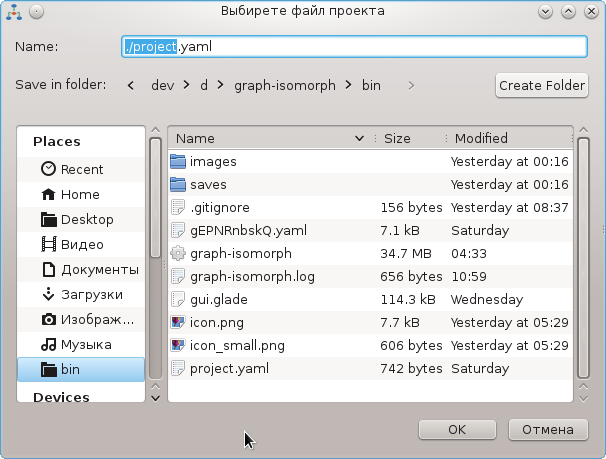
\includegraphics[width=0.5\textwidth]{screen06}
\caption{Диалог cохранения проекта}
\end{figure}

\subsection{Окно настроек}

\begin{figure}[h!]
\centering
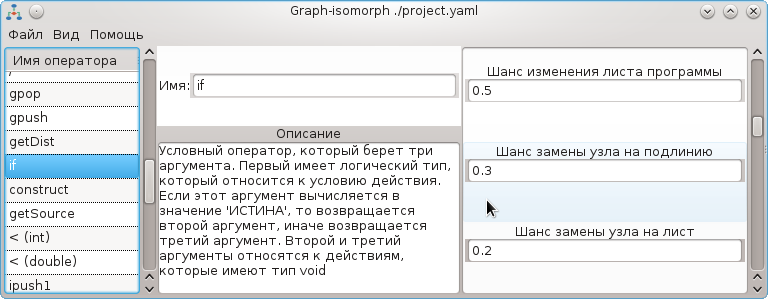
\includegraphics[width=0.8\textwidth]{screen07}
\caption{Окно настроек}
\end{figure}

Окно настроек предназначено для:
\begin{itemize}
\item Просмотра операторов проблемно-ориентированного языка, их названий и описания
\item Просмотр и установка параметров эволюции, которые сохраняются в проекте
\end{itemize}

Данное окно видно при запуске приложения, но его возможно закрыть, тогда его можно снова активировать через другие окна путем нажатия на пункт <<Показать окно настроек>> меню <<Вид>>.

\subsubsection{Просмотр операторов проблемно-ориентированного языка}
С левой стороны окна присутствует список операторов, зарегистрированных в проблемно-ориентированном языке представления алгоритмов проверки изоморфизма графов. При нажатии на имени оператора в центральной части появляется подробная информация о назначении оператора.

\subsubsection{Просмотр и установка параметров эволюции}
В правой части окна содержится список полей ввода для параметров процесса эволюции. Над каждым полем ввода имеется описание назначения параметра, в поле отображается текствовое представление параметра, которое используется АИС на данный момент. При некорректном вводе параметра появляется диалоговое окно с описанием проблемы и введенное значение отвергается.

\begin{figure}[h!]
\centering
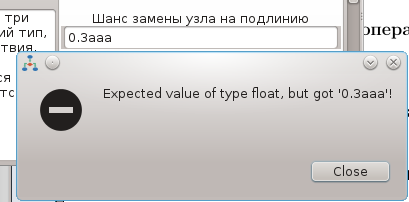
\includegraphics[width=0.5\textwidth]{screen08}
\caption{Сообщение об ошибке распознавания входных данных}
\end{figure}

\subsection{Окно эволюции}
Окно эволюции предназначено для:
\begin{itemize}
\item Отображения процесса эволюции
\item Управлением процессом эволюции
\item Просмотр входных данных для алгоритмов определения изоморфизма
\end{itemize}

При запуске приложения окно эволюции не видно, для того, чтобы активировать его, необходимо нажать на пункт <<Показать окно эволюции>> меню <<Вид>>.

\begin{figure}[h!]
\centering
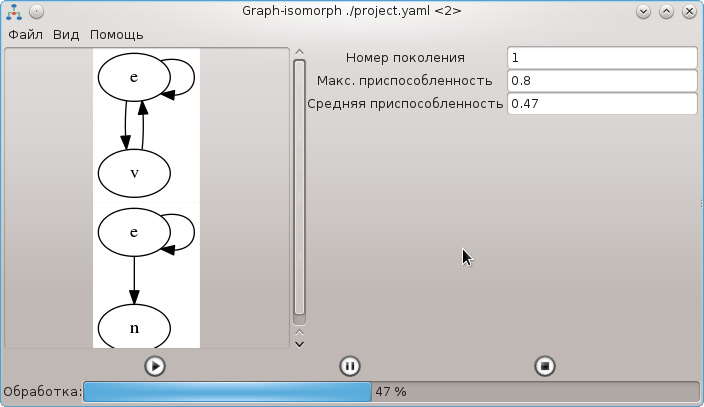
\includegraphics[width=0.8\textwidth]{screen09}
\caption{Окно эволюции}
\end{figure}

\subsubsection{Управление процессом эволюции}
В нижней части окна находится три кнопки управления процессом эволюции:
\begin{itemize}
\item Первая кнопка с черным треугольником - запуск процесса эволюции или его возобновление
\item Вторая кнопка с двумя вертикальными прямоугольниками - пауза процесса эволюции
\item Третья кнопка с черным прямоугольником - остановка процесса эволюции, при нажатии на эту кнопку будет создана новая популяция и процесс эволюции начнется с самого начала.
\end{itemize}

Также предусмотрен горизонтальный индикатор процесса обработки одного поколения. Его заполненность характеризует завершенность процессов определения значений приспособленности алгоритмов и генерации следующего поколения.

\subsubsection{Просмотр входных данных}
В левой части окна находится область отображения входных графов, которые подаются на вход проверяемых алгоритмов. Первый граф находится выше второго. Имеются полосы прокрутки для просмотра больших изображений графов.

\subsubsection{Просмотр промежуточных значений}
В правой части окна находятся поля ввода без возможности редактирования, в которых отображаются:
\begin{itemize}
\item Номер текущего поколения
\item Максимальное значение функции приспособленности
\item Среднее значение функции приспособленности
\end{itemize}


\subsection{Окно результатов}
Окно результатов предназначено для:
\begin{itemize}
\item Просмотра состава популяции
\item Просмотра исходного кода алгоритмов
\item Просмотра графической формы алгоритма
\end{itemize}

При запуске приложения окно результатов не видно, для того, чтобы активировать его, необходимо нажать на пункт <<Показать окно результатов>> меню <<Вид>>.

\begin{figure}[h!]
\centering
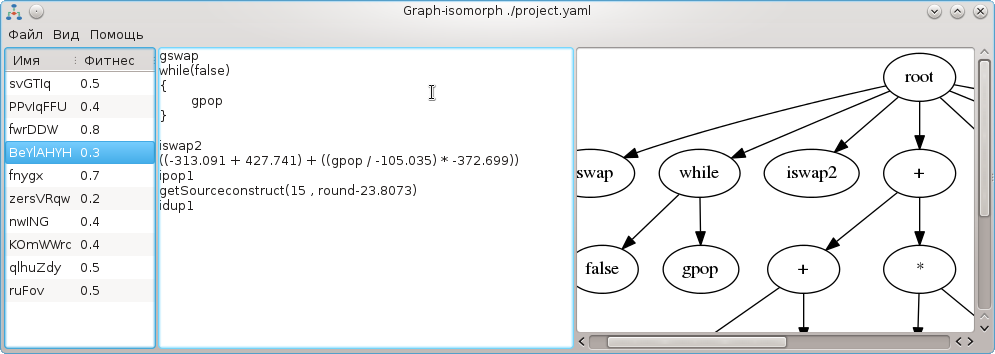
\includegraphics[width=0.9\textwidth]{screen10}
\caption{Окно результатов}
\end{figure}

\subsection{Просмотр состава популяции}
В левой части окна присутствует список индивидов, которые составляют текущую популяцию. В элемнтах списка отображается имя индивида (случайно сгенерированная строка) и значение функции приспособленности. 

\subsubsection{Просмотр исходного кода алгоритмов}
При нажатии на элемент списка индивидов в центральной области окна отображается текстовое представление генома выбранного индивида. Данный исходный код является псевдокодом с Си-подобным синтаксисом. Для длинных исходных кодов присуствуют полосы прокрутки.

\subsubsection{Просмотр графической формы алгоритма}
При нажатии на элемент списка индивидов в правой области окна отображается графическое представление генома выбранного индивида в виде дерева с переменной арностью. Для крупных изображений деревьев присуствуют полосы прокрутки.

\begin{figure}[h!]
\centering
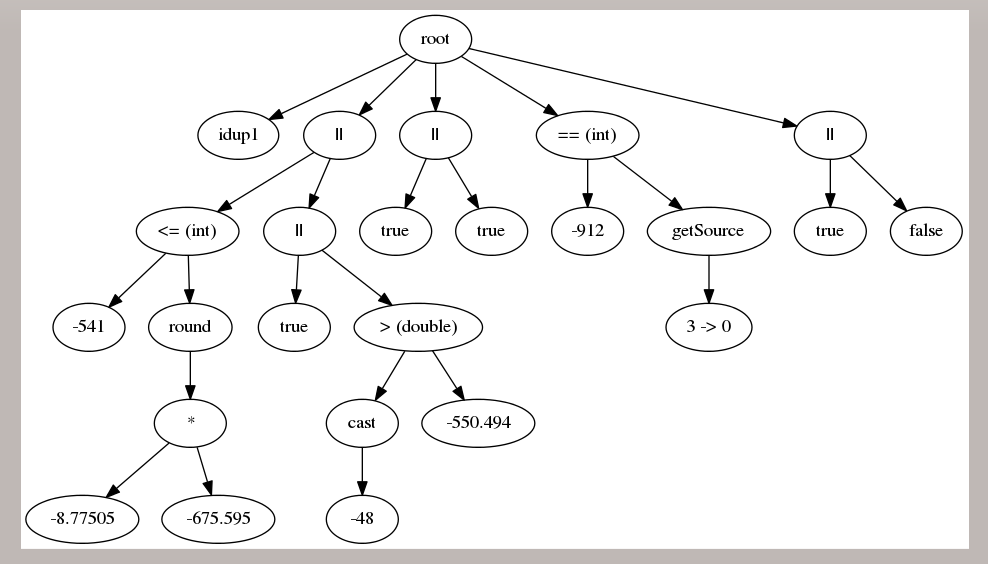
\includegraphics[width=0.9\textwidth]{screen11}
\caption{Просмотр графического представления генома индивида}
\end{figure}

\end{document}


